\documentclass[11pt]{article}

%%%%%%%%%%%%%%% PACKAGES %%%%%%%%%%%%%%%

\usepackage{url}
\usepackage{amssymb}
\usepackage{multicol}
\usepackage{enumerate}
\usepackage{tabularx}
\usepackage{graphicx}
\usepackage{amsmath}
\usepackage{amsfonts}
\usepackage{amsthm}
\usepackage{amscd}
\usepackage{amsrefs}
\usepackage[affil-it]{authblk}
\usepackage{mathtools}
\usepackage{float}


%%%%%%%%%%%%%%% TITLE/AUTHOR INFORMATION %%%%%%%%%%%%%%%

\title{Digital Signal Processing and the Gift of JPEG}
\author{Marvin Lin}
\date{\today}
\affil{Portland Community College}

%%%%%%%%%%%%%%% CUSTOM FORMAT %%%%%%%%%%%%%%%

\setlength{\textwidth}{6.5in}
\setlength{\textheight}{9in}
\setlength{\evensidemargin}{0in}
\setlength{\oddsidemargin}{0in}
\setlength{\topmargin}{+.4in}

\setlength{\oddsidemargin}{0.in}
\setlength{\evensidemargin}{0.in}
\setlength{\textwidth}{6.46in}
\setlength{\textheight}{8.4in}

\setlength{\parindent}{0pt}

\usepackage[margin=2.5cm]{geometry}

%%%%%%%%%%%%%%% PREAMBLE %%%%%%%%%%%%%%%

\newcommand{\Z}{\mathbb{Z}}
\newcommand{\Q}{\mathbb{Q}}
\newcommand{\R}{\mathbb{R}}
\newcommand{\C}{\mathbb{C}}
\DeclareMathOperator{\rank}{rank}               % Rank
\DeclareMathOperator{\vol}{vol}                 % Volume
\DeclarePairedDelimiter\abs{\lvert}{\rvert}     % Absolute Value

%%%%%%%%%%%%%%% BEGIN DOCUMENT %%%%%%%%%%%%%%%

\begin{document}

%%%%%%%%%%%%%%% TITLE %%%%%%%%%%%%%%%

\maketitle

%%%%%%%%%%%%%%% ABSTRACT %%%%%%%%%%%%%%%

\begin{abstract}

Digital signal processing (DSP) is integral to many of the computational tools we use in our everyday lives. Ranging from voice assistants, sensor data processing, to even data compression, digital processors are used regularly to perform various signal processing methods. Data is sampled in the time, space, or frequency domain and utilize linear transformations to appropriately filter and adjust the signal to specification. DSP can be seen in voice assistants such as Siri, Alexa, or Google Assistant. Voice, an analog signal, is converted with an analog-to-digital converter after data sampling, which then characterized as various commands (ie. "yes" or "no") utilizing DSP. Similarly, file and data compression software utilizes linear transformations to digitally process data to fit a smaller file size, most notably the JPEG file format.

\end{abstract}

%%%%%%%%%%%%%%% BODY OF PAPER %%%%%%%%%%%%%%%

\section{Introduction}
Signal processing may appear like a niche application of linear algebra at first glance, but in reality is a widely used approach to processing a variety of data. Signals are found across disciplines and subject areas, ranging from the the most obvious in computing and communications, to even data analysis in biomechanics \cite{book:lay}. Creating, decrypting, and processing signals are the fundamental components of signal processing. Before we can investigate the application of linear algebra in the signal processing world, we must first get a grasp of the world of signals and signal processing.

\section{Linear Algebra in Signal Processing}

\subsection{What is a signal?}

When most people hear "signal", something along the lines of "signal strength" comes to mind. By convention, we interpret the word "signal" in everyday conversation to be related to wireless communications, such as WiFi strength or phone service. However, by definition, signals are much simpler and extensive than the everyday convention.By the Google definition, signals are "a gesture, action, or sound that is used to convey information or instructions". From the sound of your voice, the flashing of lights in the dark night sky, to even neurons firing in animals like us, these all can be interpreted as signals. Understanding this, an important distinction must be made: analog vs. digital signals.\\

Digital signals are best known by the aforementioned convention. Data is represented in 1s and 0s, or better known as binary. This is how signals are processed and displayed in modern computers. On the other hand, there lies the lesser known analog signal. Analog signals are best represented in the form of graphs and waves. Most, if not all, people in the modern age have seen waveforms for audio. Instead of a representation through the binary distinction of 1/0s or on/off (finite possibilities), analog signals vary and have infinite possible values that can be represented.

\begin{figure}[H]
    \begin{center}
    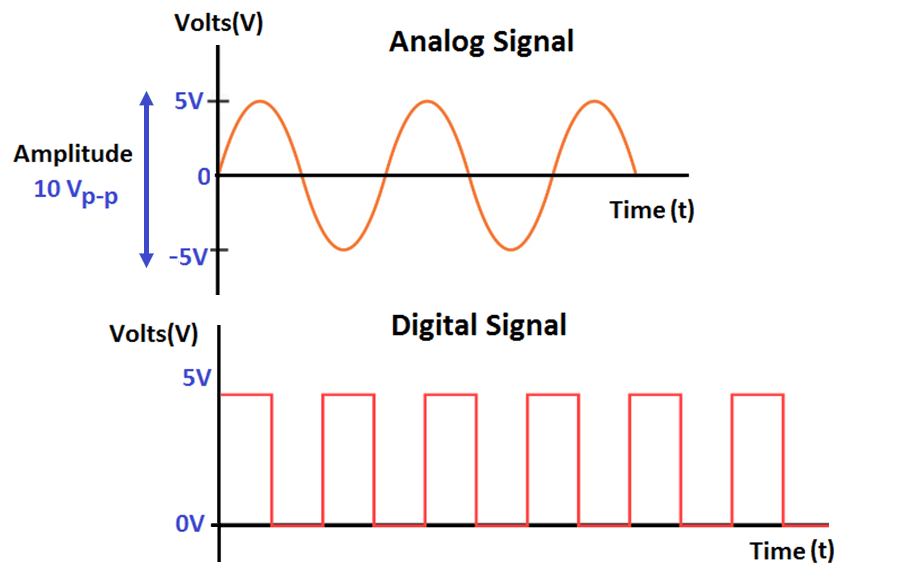
\includegraphics[width = 300px]{figures/analogVsDigital.png}
    \caption{A visual comparison of digital and analog signals \cite{website:digitalvsanalog}}
    \label{fig:analogVsDigital}
    \end{center} 
\end{figure}

As we can see, the difference in the types of signals is very apparent. This is particularly relevant when looking to understand how data is stored and encoded. Think back to an audio waveform. Clearly, the numerous values indicate that the signal is analog. However, modern computers utilize digital processors and digital storage. An analog to digital converter can be used to create a digital representation of an analog signal through a process reminiscent of a riemann sum in calculus. 

\begin{figure}[H]
    \begin{center}
    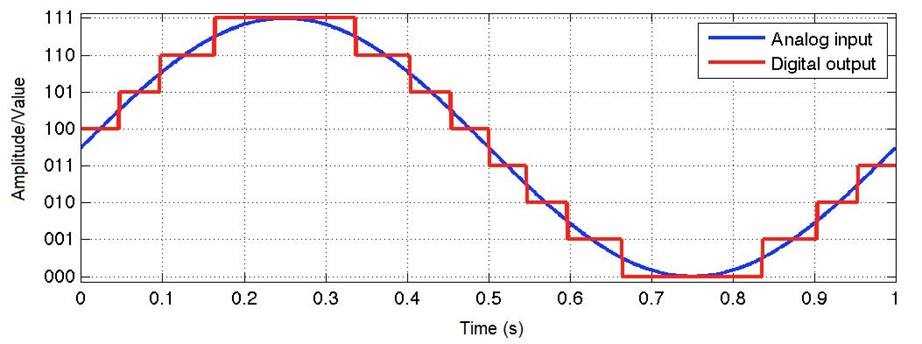
\includegraphics[width = 300px]{figures/adc.jpg}
    \caption{Conversion of an analog signal to a digital representation of a signal \cite{website:adc}}
    \label{fig:adc}
    \end{center} 
\end{figure}

When it comes to the idea of sending signals, the concept of encoding signals becomes relevant. Due to the nature of electronics and circuitry, data must be transcoded within the amplitude, phase, and frequency of a signal. All signals in the modern era are represented through alternating current, or AC. AC is best visualized through an oscillating sine wave. This is especially important to understand as modern electronics operate with alternating current in order to take advantage of AC for conveying signals. Radio frequency (RF) systems also take advantage of this to transmit information.\\

Knowing this, we can now consider encoding a signal into the oscillating currents of AC. We can do this through controlling through two common methods: amplitude modulation (AM) and frequency modulation. Sound familiar? This is because your AM and FM radios are based on these different modulation processes to encode signals within radio waves. Thinking back to radios, what is almost ALWAYS present when we turn it on? Static noise. Noise is always present in the process of conveying signals, whether it be through RF, or your hardwired connection.\\ 

Understanding this, we can start to piece together the larger picture of modern computing. When transmitting an analog signal, the noise can significantly alter the signal encoded within the oscillating waves. Therefore, analog signals are more sensitive to noise. This is why our radios are infected by static noise on a daily basis, since signals are transmitted using an analog format. This format risks data loss and miscommunication.On the other hand, digital data communication is much less susceptible to noise. Since information is encoded with two values rather than the infinite values associated with analog signals, the encoded signal is much less susceptible to noise.

\begin{figure}[H]
    \begin{center}
    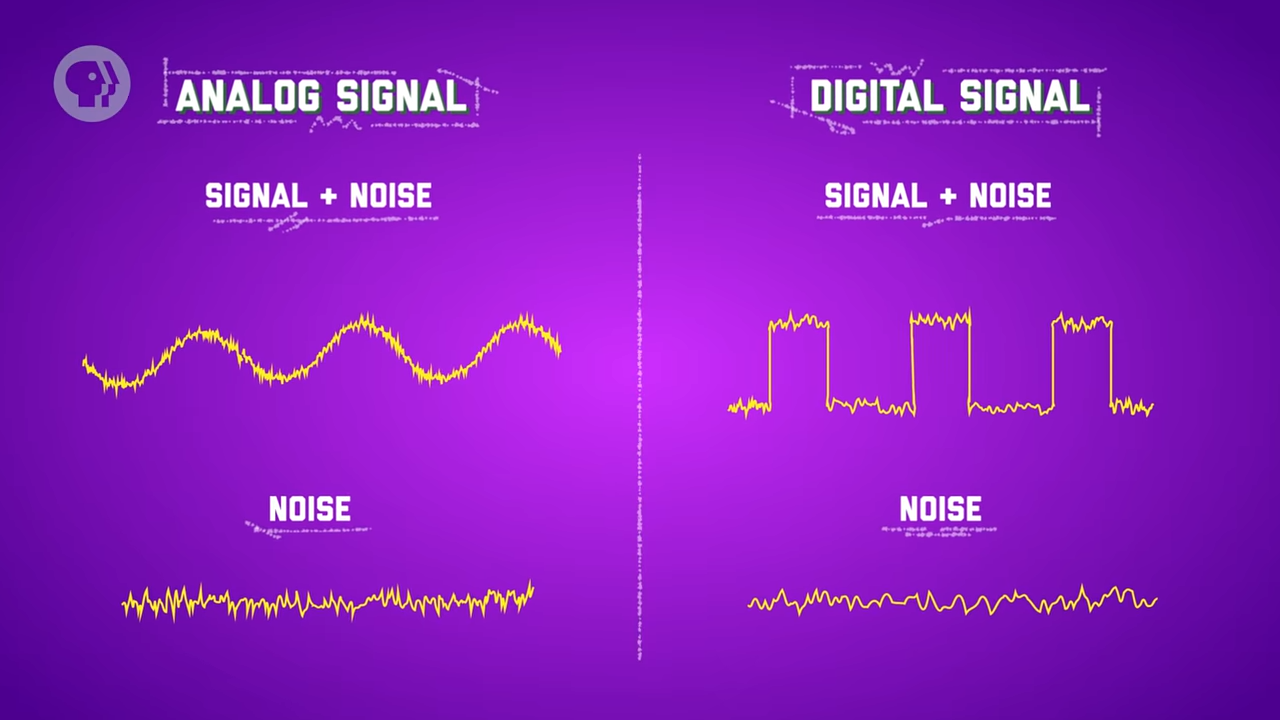
\includegraphics[width = 300px]{figures/singalAndNoise.png}
    \caption{A comparison of the impact of noise on encoded analog versus digital signals \cite{website:signalAndNoise}}
    \label{fig:singalAndNoise}
    \end{center} 
\end{figure}

With this basic understanding of signals and their fundamental purpose in real world, we can start investigating the application of linear algebra in the signal processing world.

\subsection{Discrete Time Signals: What are they?}

The space of all doubly infinite (positive and negative direction) sequences of integers is known as $\mathbb{S}$. This space is most commonly seen in understanding and measuring signals. In this space, an endless amount of signals can be created, represented in a vector. A key and commonly used signal is referred to as periodic signals. This is best characterized by a signal in which the integer value will repeat itself. Most commonly, the sinusoidal signal is often seen in everyday applications.

\subsection{Linear Time Invariant Transformations}

Fundamentally, the Linear Time Invariant Transformation (LTI) is used to process signals. This method is used to create numerous variations of signals rather than storing a variety of signals. One very common transformation used in signal processing is the shift of a signal. The concept creating signals when needed is invaluable in numerous applications, such as generation of RF signals for communication, and even when discussing file compression. This idea of creating different signals through operations that are invertible will become especially relevant in our discussion of the JPEG image compression format.

\subsection{Digital Signal Processing}

Another fundamental linear transformation is used for smoothing and filtering data, This is relevant for smoothing out stock price fluctuations and noise from communication transmissions. Since the objective of signals is to either spot trends of communicate information through trends, these transformations are undoubtedly of value in the modern world.\\

A common approach used to smooth out a signal is by taking a moving average. In taking the moving average of a data set, we can remove major fluctuations and spikes within the signal \cite{book:lay}. On the contrary, there also exists the process of Auralization. Unlike taking a moving average, auralization does the opposite. Instead of smoothing a signal, the process increases complexity of the signal with linear combinations of various signals to generate new signals. This method is most often used in the audio and entertainment industry to digitally generate audio with greater quality \cite{book:lay}.\\

It is clear that the versatility of digital signal processing allows for innumerable applications. Next, we will explore some applications of linear algebra in signal processing.

\section{Applications in the Real World}

\subsection{Voice Processing and Digital Assistants}
Applying Digital Signal Processing to voice is one of the more technologically advanced and challenge usages of DSP. The analog signal of a voice can be converted to a digital signal through an ADC, which allows the signal to take advantage of digital signal processing.\\

In the case of processing voice data for digital assistant services, the objective is to process a signal in a manner that makes patterns can be easily recognized. By utilizing the previously mentioned Linear Time Invariant transformations (LTI) to modify the converted digital signal into a "clearer" format for pattern recognition. In most cases, this involves the process of various transformations to create a smoother representation of the signal. This includes transformations such as taking a moving average.\\

Over the past decade, these trends and patterns from voice signals have been documented, allowing for digital processors to discern words, and therefore allowing searches and commands to be triggered. Moreover, these assistants are often able to identify commands and requests in noise conditions humans would typically not be able to discern words from, all thanks to the process of smoothing out signals for pattern recognition.

\subsection{JPEG Compression: Too good to be true!}
While concepts around Digital Signal Processing may be associated with more "typical" signals such as data from an analog sensor or processing of audio data, the applications of DSP applies to far more. Various other forms of data, such as images, can also be reduced down to signals, allowing various transformations and processes to occur in order to get the desired end product.

\subsubsection{Understanding Image Compression Basics}

Traditionally, the size of a raw image file often is very large, often impractical for portability across various devices. To resolve this, image compression methods are utilized to reduce data while maintaining the visual quality of the original. The concept itself is utilizes a combination of transformations with an understanding of human physiology and psychology to determine the most effective approach to image compression.\\

Two main forms of compression exist: lossy and lossless compression. Like the names imply lossy compression indicates the loss of information from the raw file, which in turn allows for greater compressibility. Lossless compression allows all information to be kept, however often at the sacrifice of compressibility. The JPEG image format is a form of lossy image compression, which allows file sizes to be reduced significantly.\\

In designing the JPEG format, several factors were considered. First and foremost, the design considered human psychology. Humans are able to discern a limited amount of from an image, which allows the usage of lossy compression to be used. More specifically, humans are more sensitive to brightness than colors \cite{website:jpeg}. JPEG is designed to be a practical and portable compression method while still maintaining a high level of quality. In this next section, we will explore how the JPEG format maintains a high level of resolution and quality despite massive data savings.

\subsubsection{Reducing an Image to Signals}

To begin this process, we need to start by reducing an image into a processable signal. This can be done by analyzing the rows of pixels as values to be plotted on a graph. Let's start with a black and white image for simplicity.

\begin{figure}[H]
    \begin{center}
    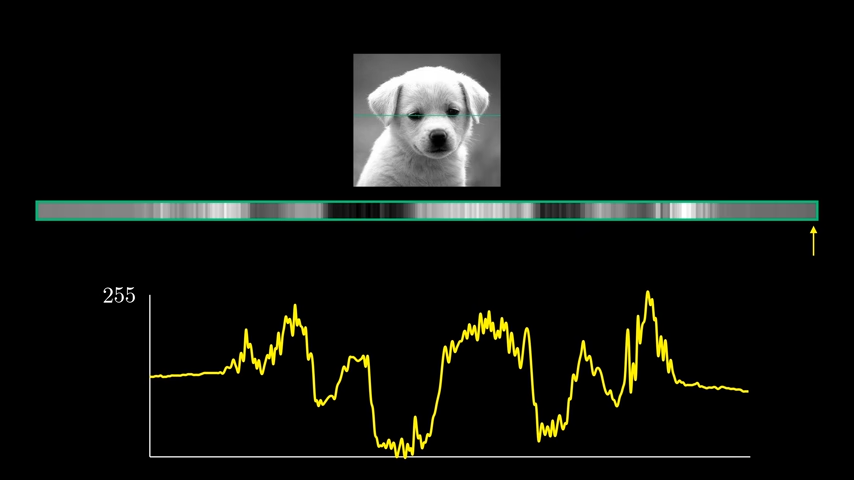
\includegraphics[width = 300px]{figures/jpegSignal.png}
    \caption{Images represented as a signal from \cite{website:jpeg}}
    \label{fig:jpegSignal}
    \end{center} 
\end{figure}
    
Images are represented through the RGB color-space, which spans 255 different variations of the colors. In reducing the image down to black and white, we have effectively reduced the problem from one in $\R^3$ to one in $\R^1$. We can then create a graph of the variations of shade to create signal.\\

Creating this representation of the pixels of an image in signal form, we can begin analyzing the various components of the image. One area of focus by the JPEG designers was the impact of frequency in the signal, or how often the signal has a significant change in color. Turns out, real world images tend to have more lower frequency components than high, and humans tend to be far less sensitive to higher frequency detail. The human brain appears to average this information anyways. Understanding this, we can reduce data size by removing data on the high frequency components of the image. To do this, we first need to get the frequency component from the image.

\subsubsection{The Discrete Cosine Transform}

The process of the discrete cosine transforms focuses on recreating the signal with a linear combination of various cosine functions. As previously explored, we know that any function can be recreated as a linear combination of cosine functions. In identifying these cosine functions, analysis and processing of the signal can be completed. One important factor to consider in the discrete cosine transform is that it only focuses on the discrete values that are relevant to the image itself. While the shape of the graph may be helpful to visualize, the only relevant information truly lies in the discrete points.

\begin{figure}[H]
    \begin{center}
    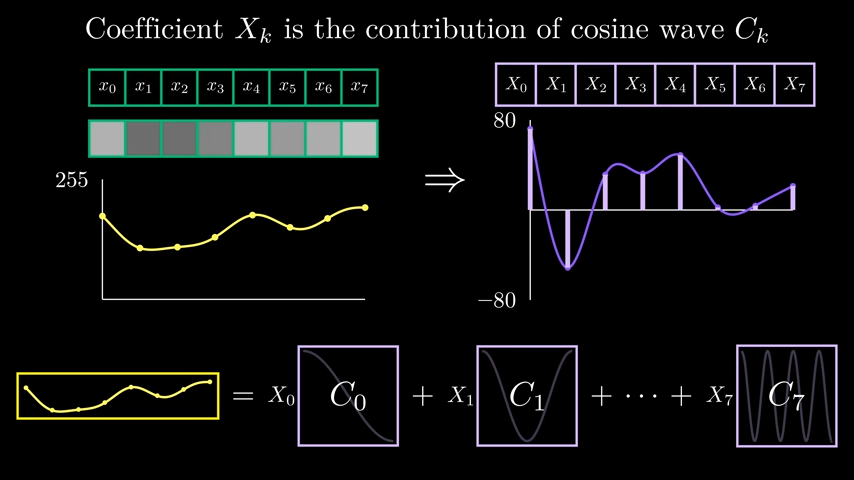
\includegraphics[width = 300px]{figures/jpegDCT.png}
    \caption{Visualization of the Discrete Cosine Transform (DCT) \cite{website:jpeg}}
    \label{fig:jpegDCT}
    \end{center} 
\end{figure}

So how do we reach this? We can analyze the frequency by reducing the complex signal into a linear combination of cosine functions. All singals, one way or another, can be defined by linear combination of cosine functions. With this method, we are able to determine the weight of various cosine functions, as modeled in the image above as $X_k$. Moreover, we can mathematically represent this by the sum of all relevant cosine functions:\\

\begin{center}
    $
    X_k=\sum_{n = 0}^{N-1}x_n\cos \left[ \frac{(2n+1)\pi k}{2N} \right] \Longleftrightarrow X_k=\mathbf{C^T_k}\cdot \mathbf{x}
    $ \cite{website:jpeg}
\end{center}

The resulting summation can be simplified down to something very familiar: a dot product. We know that a dot product is used to determine similarity between vectors in relation to each other. In essence, we can represent the DCT with a simple dot product. We can better visualize this as simply a matrix vector product in order to transform a set of sampled points to a linear combination of cosine functions:

\begin{center}
    $
    \begin{bmatrix}
        X_0 \\
        X_1 \\
        X_2 \\
        X_3 \\
        X_4 \\
        X_5 \\
        X_6 \\
        X_7
    \end{bmatrix}
    =
    \begin{bmatrix}
        \longleftarrow C^T_0 \longrightarrow \\
        \longleftarrow C^T_1 \longrightarrow \\
        \longleftarrow C^T_2 \longrightarrow \\
        \longleftarrow C^T_3 \longrightarrow \\
        \longleftarrow C^T_4 \longrightarrow \\
        \longleftarrow C^T_5 \longrightarrow \\
        \longleftarrow C^T_6 \longrightarrow \\
        \longleftarrow C^T_7 \longrightarrow
    \end{bmatrix}
    \begin{bmatrix}
        x_0 \\
        x_1 \\
        x_2 \\
        x_3 \\
        x_4 \\
        x_5 \\
        x_6 \\
        x_7
    \end{bmatrix}
    $ \cite{website:jpeg}
\end{center}

This is the beauty of JPEG. Images can be reduced down to linear combinations of cosine functions, which can be determined by a simple matrix-vector product. This information can then be used to further compress the information of the JPEG format into a much smaller package while retaining quality. While there is far more to understanding the mathematical complexity and beauty of the JPEG image format, we can see how fundamental concepts of linear algebra is to encoding and decoding the compression for JPEG.

\section{Conclusion}

The applications of linear algebra in the world of signal processing is truly incredible. By understanding the space of a signal ($\mathbb{S}$), the linear time invariant transformations, and their applications in the world of digital signal processing, we can begin to analyze the beautifully complex math involved in advanced technology, from JPEG to voice assistants. However, the application of signal processing is not limited to these technologies. Once a signal can be formed, the possibilities of processing the signal is endless with DSP.

%%%%%%%%%%%%%%% BIBLIOGRAPHY %%%%%%%%%%%%%%%

\bibliographystyle{plain}
\bibliography{refs}

%%%%%%%%%%%%%%% END DOCUMENT %%%%%%%%%%%%%%%

\end{document} 